\documentclass{beamer}
\mode<presentation>
\usepackage{amsmath,amssymb,mathtools}
\usepackage{textcomp}
\usepackage{gensymb}
\usepackage{adjustbox}
\usepackage{subcaption}
\usepackage{enumitem}
\usepackage{multicol}
\usepackage{listings}
\usepackage{url}
\usepackage{graphicx} % <-- needed for images
\def\UrlBreaks{\do\/\do-}

\usetheme{Boadilla}
\usecolortheme{lily}
\setbeamertemplate{footline}{
  \leavevmode%
  \hbox{%
  \begin{beamercolorbox}[wd=\paperwidth,ht=2ex,dp=1ex,right]{author in head/foot}%
    \insertframenumber{} / \inserttotalframenumber\hspace*{2ex}
  \end{beamercolorbox}}%
  \vskip0pt%
}
\setbeamertemplate{navigation symbols}{}

\lstset{
  frame=single,
  breaklines=true,
  columns=fullflexible,
  basicstyle=\ttfamily\tiny   % tiny font so code fits
}

\numberwithin{equation}{section}

% ---- your macros ----
\providecommand{\nCr}[2]{\,^{#1}C_{#2}}
\providecommand{\nPr}[2]{\,^{#1}P_{#2}}
\providecommand{\mbf}{\mathbf}
\providecommand{\pr}[1]{\ensuremath{\Pr\left(#1\right)}}
\providecommand{\qfunc}[1]{\ensuremath{Q\left(#1\right)}}
\providecommand{\sbrak}[1]{\ensuremath{{}\left[#1\right]}}
\providecommand{\lsbrak}[1]{\ensuremath{{}\left[#1\right.}}
\providecommand{\rsbrak}[1]{\ensuremath{\left.#1\right]}}
\providecommand{\brak}[1]{\ensuremath{\left(#1\right)}}
\providecommand{\lbrak}[1]{\ensuremath{\left(#1\right.}}
\providecommand{\rbrak}[1]{\ensuremath{\left.#1\right)}}
\providecommand{\cbrak}[1]{\ensuremath{\left\{#1\right\}}}
\providecommand{\lcbrak}[1]{\ensuremath{\left\{#1\right.}}
\providecommand{\rcbrak}[1]{\ensuremath{\left.#1\right\}}}
\theoremstyle{remark}
\newtheorem{rem}{Remark}
\newcommand{\sgn}{\mathop{\mathrm{sgn}}}
\providecommand{\abs}[1]{\left\vert#1\right\vert}
\providecommand{\res}[1]{\Res\displaylimits_{#1}}
\providecommand{\norm}[1]{\lVert#1\rVert}
\providecommand{\mtx}[1]{\mathbf{#1}}
\providecommand{\mean}[1]{E\left[ #1 \right]}
\providecommand{\fourier}{\overset{\mathcal{F}}{ \rightleftharpoons}}
\providecommand{\system}{\overset{\mathcal{H}}{ \longleftrightarrow}}
\providecommand{\dec}[2]{\ensuremath{\overset{#1}{\underset{#2}{\gtrless}}}}
\newcommand{\myvec}[1]{\ensuremath{\begin{pmatrix}#1\end{pmatrix}}}
\let\vec\mathbf

\title{MatGeo Presentation - Problem 10.7.8}
\author{EE25BTECH11064 - Yojit Manral}
\date{}

\begin{document}

\frame{\titlepage}
\begin{frame}{Question}
The area (in sq. units) of the quadrilateral formed by the tangents at the end points of the latera recta to the ellipse $\frac{x^2}{9} + \frac{y^2}{5} = 1$ is
\begin{enumerate}[label=(\alph*)]
\begin{multicols}{4}
    \item $\frac{27}{2}$
    \item $27$
    \item $\frac{27}{4}$
    \item $18$
\end{multicols}
\end{enumerate}
\end{frame}

\begin{frame}{Solution}
$\rightarrow$ The parameters of the given conic are
\begin{align}
    \vec{V} = \myvec{5/9&0\\0&1}\text{, } \vec{u} = 0\text{, } f = -5
\end{align}
$\rightarrow$ Also, using eigenvalue decomposition
\begin{align}
    \vec{P} = \myvec{1&0\\0&1}\text{, } \vec{D} = \myvec{5/9&0\\0&1} \implies \lambda_1 = 5/9\text{ and } \lambda_2 = 1
\end{align}
$\rightarrow$ This gives us very useful information
\begin{align}
    e &= \sqrt{1-\frac{\lambda_1}{\lambda_2}} = \frac{2}{3} \\
    \vec{F} &= \pm e\sqrt{\frac{\vert\vec{u}^T\vec{V}^{-1}\vec{u}-f\vert}{\lambda_2(1-e^2)}}\vec{e_1} = \pm\myvec{2\\0}
\end{align}
$\rightarrow$ Given that the points of contact are the end points of the latera recta. In the first quadrant, we have
\begin{align}
    \vec{q} = \myvec{2\\5/3}
\end{align}
\end{frame}

\begin{frame}{Solution}
$\rightarrow$ If the point of contact is $\vec{q}$, the equation of tangent to the conic is
\begin{align}
    (\vec{V}\vec{q}+\vec{u})^T\vec{x} + \vec{u}^T\vec{q} + f = 0\\
    \implies \myvec{2&3}\vec{x} = 9 
\end{align}
$\rightarrow$ Thus, we get the area of the quadrilateral in the $1^{st}$ quadrant to be
\begin{align}
    \Delta_1 &= \text{Area of }\triangle = \frac{1}{2}x_{int}y_{int} = \frac{1}{2}\times\frac{9}{2}\times3 \\
    \Delta_1 &= \frac{27}{4} sq. units
\end{align}
$\rightarrow$ Since an ellipse has a two-fold symmetry, total area of the quadrilateral must be $4$ times the area in the $1^{st}$ quadrant
\begin{align}
    \Delta_{Total} = 4\times\Delta_1 = 27 sq. units
\end{align}
$\rightarrow$ Therefore, (b) 27 is the correct option
\end{frame}

\begin{frame}{Solution}
\begin{figure}[h!]
   \centering
   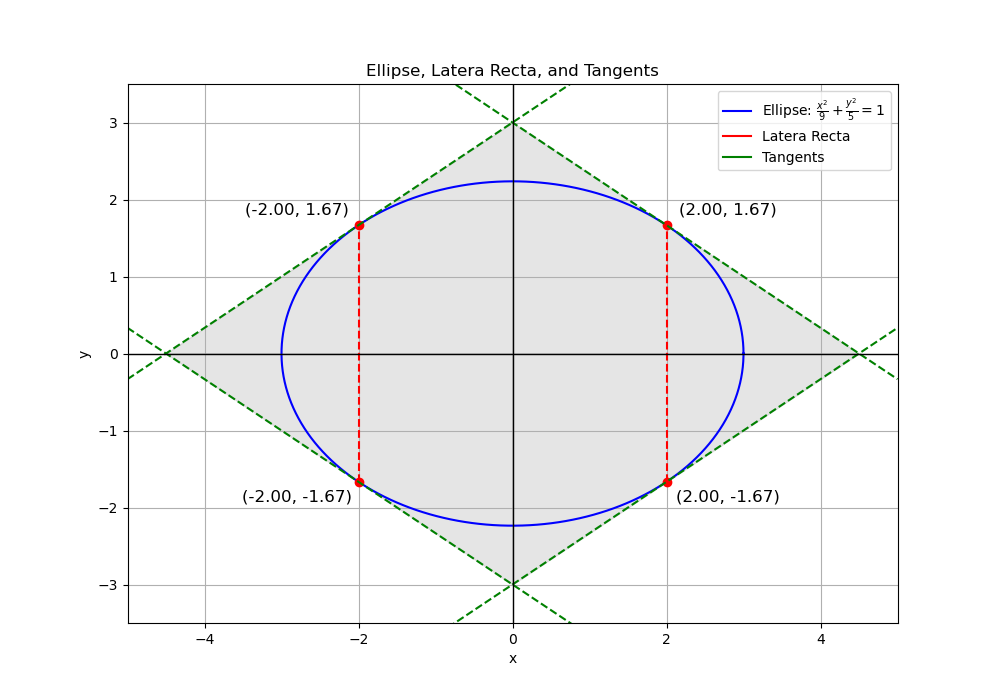
\includegraphics[width=0.9\linewidth]{figs/01.png}
   \caption{Plot of ellipse and quadrilateral}
   \label{Plot_1}
\end{figure}
\end{frame}
 % --------- CODE APPENDIX ---------
\section*{Appendix: Code}
% Python plotting
\begin{frame}[fragile]{File: plot.py}
\begin{lstlisting}[language=Python]
import numpy as np
import matplotlib.pyplot as plt
from matplotlib.lines import Line2D

# Ellipse parameters
a = 3  # semi-major axis
b = np.sqrt(5)  # semi-minor axis

# Generate points for the ellipse
theta = np.linspace(0, 2 * np.pi, 400)
x = a * np.cos(theta)
y = b * np.sin(theta)

# Points for the latus rectum
latus_rectum_points = [(2, 5/3), (2, -5/3), (-2, 5/3), (-2, -5/3)]

# Tangent line equation function
def tangent_line(x1, y1):
    """Return the equation of the tangent line at (x1, y1) on the ellipse."""
    return lambda x: (1 - (x * x1 / a**2)) * (b**2 / y1)

# Set up the plot
fig, ax = plt.subplots(figsize=(8, 8))

# Plot the ellipse
ax.plot(x, y, color="blue")
ellipse = Line2D([0], [0], color='b')
\end{lstlisting}
\end{frame}

\begin{frame}[fragile]{File: plot.py}
\begin{lstlisting}[language=Python]
#Mark the Latera Recta
ax.plot([2, 2], [-5/3, 5/3], 'r--')
ax.plot([-2, -2], [-5/3, 5/3], 'r--')
latera_recta = Line2D([0], [0], color='r', linestyle='-')

# Mark and label the latus rectum points with two decimal places
for (x1, y1) in latus_rectum_points:
    ax.plot(x1, y1, 'ro')  # Mark the point
    ax.text(x1+0.8*(x1/np.abs(x1)), y1+0.2*(y1/np.abs(y1)), f'({x1:.2f}, {y1:.2f})', fontsize=12, ha='center', va='center')

# Plot tangents at the endpoints of the latus rectum
for (x1, y1) in latus_rectum_points:
    # Get tangent function
    tangent = tangent_line(x1, y1)
    
    # Create x values for the tangent lines
    x_vals = np.linspace(-5, 5, 100)
    y_vals = tangent(x_vals)  # Calculate corresponding y values
    
    # Plot the tangent lines
    ax.plot(x_vals, y_vals, 'g--')
    
    #Fill in the quadrilateral
    quad_x = np.linspace(0, 4.5, 90) if x1>0 else np.linspace(-4.5, 0, 90)
    quad_y1 = tangent(quad_x)
    plt.fill_between(quad_x, quad_y1, color='gray', alpha=0.2)
tangents = Line2D([0], [0], color='g', linestyle='-')
\end{lstlisting}
\end{frame}

\begin{frame}[fragile]{File: plot.py}
\begin{lstlisting}[language=Python]
# Set axes limits
ax.set_xlim(-5, 5)
ax.set_ylim(-3.5, 3.5)

# Add labels and title
ax.set_xlabel("x")
ax.set_ylabel("y")
ax.axhline(0, color='black', linewidth=1)
ax.axvline(0, color='black', linewidth=1)
ax.set_title("Ellipse, Latera Recta, and Tangents")

# Show grid
ax.grid(True)

# Show the plot
plt.legend(handles=[ellipse, latera_recta, tangents], labels=['Ellipse: $\\frac{x^2}{9} + \\frac{y^2}{5} = 1$', 'Latera Recta', 'Tangents'])
plt.gca().set_aspect('equal', adjustable='box')
plt.show()
\end{lstlisting}
\end{frame}
\end{document}
